\documentclass{beamer}
  \usepackage[english]{babel}
  \usepackage[utf8]{inputenc}
  \usepackage{times}
  \usepackage[poster]{tcolorbox}
  \usepackage{fontawesome}
  \usepackage{fontspec}
  \usepackage{amsmath,amsthm, amssymb, latexsym}
  \boldmath

    
  \usetheme{Sharelatex}
  \usepackage[orientation=portrait,size=a0,scale=1.4]{beamerposter}
  \setbeamersize{text margin left=0mm,text margin right=0mm} 

  \title[ITS low temperature plasma]{Incoherent Thomson Scattering (ITS) applied to low temperature plasma sources}
  \author[benjamin.vincent@cnrs-orleans.fr]{Benjamin Vincent}
  \institute[CNRS]{ICARE Laboratory, CNRS Orléans}
  \date{\today}
  
  \logo{
\includegraphics[height=.06\paperwidth]{logo-cnrs-simple}}


  %%%%%%%%%%%%%%%%%%%%%%%%%%%%%%%%%%%%%%%%%%%%%%%%%%%%%%%%%%%%%%%%%%%%%%%%%%%%%%%%%5

  \begin{document}
  \begin{frame}{} 
  
\vspace{0.02\paperwidth}

\begin{tcbposter}[
   poster = {showframe , columns=100,rows=2,colspacing=0mm , rowspacing=0.01\paperwidth , height=0.3\paperwidth , width=\paperwidth},
   no coverage ,
   boxes = {beamer,arc=10mm,colback=bleuet, colframe=bleuet, no shadow}
   ]
 
  \posterbox[adjusted title= \color{beige} \faDotCircleO \ Introduction \faDotCircleO, sharp corners = northeast, sharp corners = southeast, sharp corners = southwest]{name=Intro,column=3,row=1,span=34}{ 
   \color{beige} 
   \small  
	Low-temperature plasma sources offers wide ranges of applications such as electric propulsion, thin film deposition, particles sources for accelerators, ...  Behaviors of such plasmas being strongly correlated to electron properties, reliable diagnostics are needed to probe electrons. These experimental results are needed to increase our understanding of the physics of such complex plasma sources and validate predictive simulations under development.	
	 } 
 
  \posterbox[adjusted title= \color{beige} \faDotCircleO \ Aim \faDotCircleO, sharp corners = northeast, sharp corners = southeast, sharp corners = southwest]{name=Motiv,column=3,row=2,span=34}{ 
   \color{beige} 
   \small 
In this work we prove that Incoherent Thomson scattering measurements using a monochromator and Volume Bragg Grating based Notch Filters (VBG-NF) can compete with the performance obtained with Triple Grating Spectrometer (TGS). Electron properties measurement with spatial resolution down to $0.3 \ \mu m$ and possible temporal measurement down to $1\mu s$ were performed on cathode and magnetron sources with temperature ranging from $0.5 \ eV$ to $20 \ eV$ and electron density from $10^{16} \ m^{-3}$ to $10^{18} \ m^{-3}$.	
	 } 
 
  \posterbox[adjusted title=\color{beige} \faDotCircleO \ Method \faDotCircleO , sharp corners = northwest, sharp corners = southwest]{name=Meth,column=38,row=1,span=60,rowspan=2}{ 
  	\color{beige} 
	\small
	
\begin{columns}
	\begin{column}{0.38\paperwidth}
	Incoherent Thomson scattering involves the observation of scattering of photons by free charged particles (electrons in our study) at length scales smaller than the screening Debye length. A these length scales individual electrons properties modulate scattered photon properties. Averaged over the scattering volume and the solid angle of observation, the photon spectral intensity measured in the case of a Maxwellian Electron Velocity Distribution Function (EVDF) can be expressed as:
	\begin{equation}
	I_{T}(\lambda,\Delta \lambda_{g}, \lambda_{0},n_{e})=c_{1}n_{e} P_{i}L\delta \lambda \frac{d \sigma_{T}}{d \Omega}(\theta, \phi) \left( \frac{e^{- \frac{(\lambda-\lambda_{0})^{2}}{2 \Delta \lambda_{g}^{2}}}}{\Delta \lambda_{g} \sqrt{2 \pi}} \ast I \right) (\lambda) 	
	\end{equation}
	\end{column}

	\begin{column}{0.22\paperwidth}
	\begin{figure}
	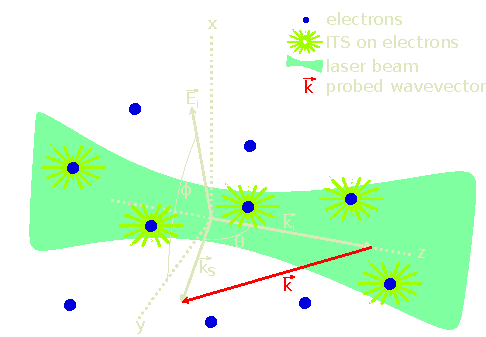
\includegraphics[width=0.2\paperwidth]{Scattering_Configuration_angles_bright.pdf}
	\end{figure}
	\end{column}
\end{columns}
		
	With $c_{1}$ the total transmission factor obtained after a Raman calibration, $P_{i}$ the laser power, $L$ the length of the scattering volume, $\delta \lambda$ the wavelength width cover by each pixel of the detector, $\frac{d \sigma_{T}}{d \Omega}(\theta, \phi)= r_{e}^{2}(1-sin^{2}\theta cos^{2} \phi)$ the differential Thomson scattering cross section int the observation direction and $I(\lambda)$ the norme instrument function of the detection branch.From the spectrum fitting is $n_{e}$ is directly obtained, $\Delta \lambda_{g}$ gives $T_{e}$ and $\lambda{0}-\lambda_{i}$ gives $v_{e,drift}$.
	
	In case of low noise Thomson signals, the Electron Energy Distribution Function (EEDF) can be extracted from the normed derivative of the spectral intensity: $f_{E}(E) \propto \frac{dI}{d\lambda}$ with $E=\frac{m_{e}}{2} \cdot \frac{c (\lambda-\lambda_{0})}{2 \lambda_{i} sin(\theta/2)}$.
 } 
 \end{tcbposter}

%%%%%%%%%%%%%%%%%%%%%%%%%%%%%%%%%%%%%%%%%%%%%%%%%%%%%%%%%%%%%%%%%%%%%%%%%%%%%%%%%%%%%%%%%%%%%%%%%%%
%%%%%%%%%%%%%%%%%%%%%%%%%%%%%%%%%%%%%%%%%%%%%%%%%%%%%%%%%%%%%%%%%%%%%%%%%%%%%%%%%%%%%%%%%%%%%%%%%%%    
\vspace{.02\paperwidth}    
%%%%%%%%%%%%%%%%%%%%%%%%%%%%%%%%%%%%%%%%%%%%%%%%%%%%%%%%%%%%%%%%%%%%%%%%%%%%%%%%%%%%%%%%%%%%%%%%%%%
%%%%%%%%%%%%%%%%%%%%%%%%%%%%%%%%%%%%%%%%%%%%%%%%%%%%%%%%%%%%%%%%%%%%%%%%%%%%%%%%%%%%%%%%%%%%%%%%%%%
\begin{tcbposter}[
   poster = {showframe , columns=100,rows=2,colspacing=0mm , rowspacing=0.01\paperwidth , height=0.6\paperwidth , width=\paperwidth},
   no coverage ,
   boxes = {beamer,arc=10mm,colback=bleuet, colframe=bleuet, no shadow}
   ]
 
  \posterbox[adjusted title= \color{beige} \faDotCircleO \ Experimental setup \faDotCircleO,title , sidebyside , righthand ratio=0.58,  sharp corners = northeast, sharp corners = northwest]{name=Exp,column=3,row=1,span=96}{ 
   \color{beige} 
   \small 
        		\textsc{Transmission branch:}
     		\begin{itemize}
     			\item Q-switch Nd:YAG laser ($\lambda_{i}=....532 \ nm; \ \tau=5 \ ns$, $10 \ Hz$, $430 \ mJ$)
     			\item Brewster windows far from the observation volume and apertures
     			\item Waist $w_{0}\approx 0.3 \ mm$
     			\item Large aperture beam dump
     		\end{itemize}
     		
     		\textsc{Detection branch:}
     		\begin{itemize}
     			\item Fiber bundle ($5 \times 3$, $0.3 \mu m$)
     			\item Volume Bragg Grating based Notch Filter (VBG-NF)
     			\item Acton SP-2750 spectrometer
     			\item ICCD PI-MAX 5 camera (gen II intensifier)
     		\end{itemize} 
     		
$\Rightarrow$ Result    
     		
\tcblower

	 	\begin{figure}
	 		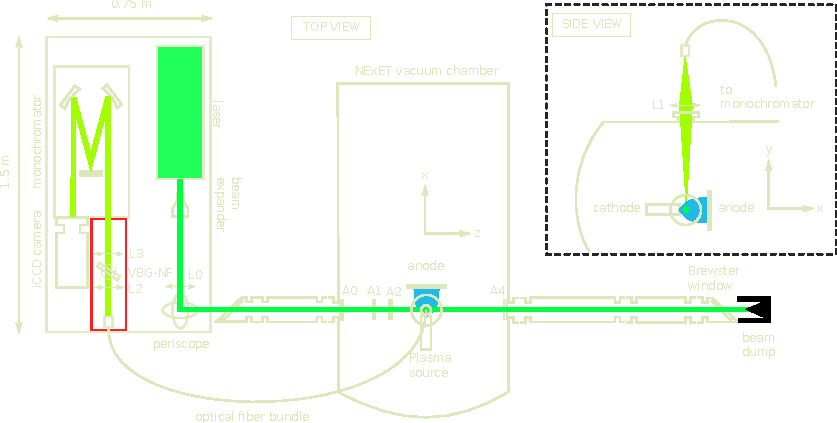
\includegraphics[width=0.545\paperwidth]{THETIS_on_NEXET_bright.pdf}
	 	\end{figure}	
     		
     		
   } 
   
   \posterbox[adjusted title= \color{beige} \faDotCircleO \ Results \faDotCircleO, sharp corners = southeast, sharp corners = southwest]{name=Results,column=3,row=2,span=96}{ 
   \color{beige} 
   \small 
   } 
   \end{tcbposter}	
	 
%\begin{columns}[t] 
%	
%	\begin{column}{.02\paperwidth}
%	\end{column} 
%
%	\begin{column}{.96\paperwidth}
%     
%       \begin{tcolorbox}[title= \color{beige} \faDotCircleO \ Experimental setup \faDotCircleO,  width=.96\paperwidth, arc=10mm, colback=bleuet, colframe=bleuet]%{headline}
%     \vspace{.0075\paperwidth} 
%     \small
%     \color{beige}
%     \begin{columns}
%     		\begin{column}{.0075\paperwidth}
%     		\end{column} 
%     		     
%     		\begin{column}{.4\paperwidth}
%     		\textsl{Transmission branch:}
%     		\begin{itemize}
%     			\item Q-switch Nd:YAG laser ($\lambda_{i}=....532 \ nm; \ \tau=5 \ ns$, $10 \ Hz$, $430 \ mJ$)
%     			\item Brewster windows far from the observation volume and apertures
%     			\item Waist $w_{0}\approx 0.3 \ mm$
%     			\item Large aperture beam dump
%     		\end{itemize}
%     		
%     		Detection branch:
%     		\begin{itemize}
%     			\item Fiber bundle ($5 \times 3$, $0.3 \mu m$)
%     			\item Volume Bragg Grating based Notch Filter (VBG-NF)
%     			\item Acton SP-2750 spectrometer
%     			\item ICCD PI-MAX 5 camera (gen II intensifier)
%     		\end{itemize}     		
%     		
%$Rightarrow$ result     		
%     		
%     		\end{column} 
%
%     		\begin{column}{.545\paperwidth}
%	 	\begin{figure}
%	 		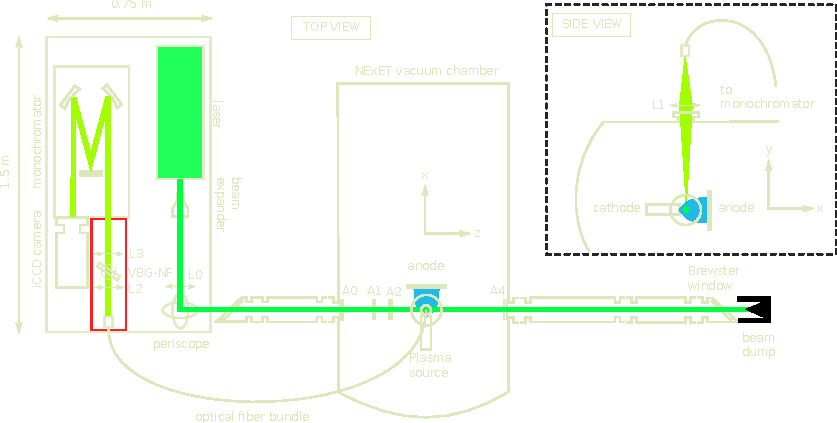
\includegraphics[width=0.545\paperwidth]{THETIS_on_NEXET_bright.pdf}
%	 	\end{figure}	       
%         	\end{column}    
%         	
%
%     		\begin{column}{.0075\paperwidth}
%     		\end{column}      	      
%       \end{columns}
%       
% 	 \end{tcolorbox}
% 	
% 	\vspace{.02\paperwidth}
%
%       \begin{tcolorbox}[title= \color{beige} \faDotCircleO \ Results \faDotCircleO, height=.5\paperwidth , width=.96\paperwidth, arc=10mm, colback=bleuet, colframe=bleuet]%{headline}
%       \vspace{.0075\paperwidth} 
%       \color{beige} 
%       \small
%       
% 	 \end{tcolorbox}
% 	  \end{column} 
% 	  
% 	 \begin{column}{.02\paperwidth}
%      \end{column} 
%
%\end{columns}  
%    
\end{frame}

\end{document}


%%%%%%%%%%%%%%%%%%%%%%%%%%%%%%%%%%%%%%%%%%%%%%%%%%%%%%%%%%%%%%%%%%%%%%%%%%%%%%%%%%%%%%%%%%%%%%%%%%%%
%%% Local Variables: 
%%% mode: latex
%%% TeX-PDF-mode: t
%%% End:
